\begin{figure}
  \centering
    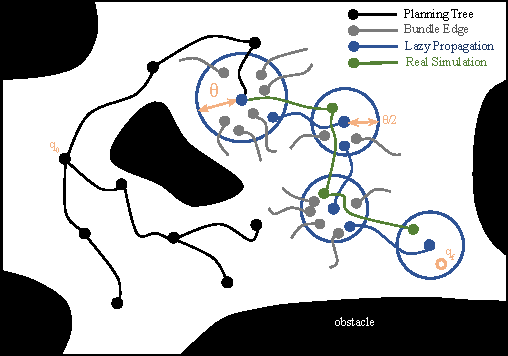
\includegraphics[width=\columnwidth,height=0.7\columnwidth]{assets/theta_over_2.pdf}
  \caption{\textsl{LazyBoE} can lazily propagate a series of edges from $\mathcal{E}$ (shown in \textsl{grey}) in a way that minimizes heuristic cost. After a lazy candidate path is found (\textsl{blue}), a full simulation and collision check is performed along this path (\textsl{green}) to extend the planning tree (\textsl{black}). To ensure the highest rate of success when performing simulation on lazy paths, neighborhood lookup is restricted to $\theta / 2$ for lazy search to allow, in the worst case, the maximum error between the end of a simulated edge and the start of the next lazy edge to be $\theta$.}\label{fig:theta_over_2}
\end{figure}